% The running example of Section 2.1 under do(X_2 = theta): no arrows into X_2, U_2 removed.
% Compile on its own (pdflatex intervention_on_X2.tex); the thesis includes the PDF.
% The invisible node in place of U_2 keeps the same size as scm-running-example.pdf and
% intervention_on_X1-example.pdf, so all three are drawn at the same scale.
\documentclass[12pt,border=2pt]{standalone}
\usepackage[T1]{fontenc}
\usepackage{mathpazo}
\usepackage{tikz}
\usetikzlibrary{arrows.meta}
\begin{document}
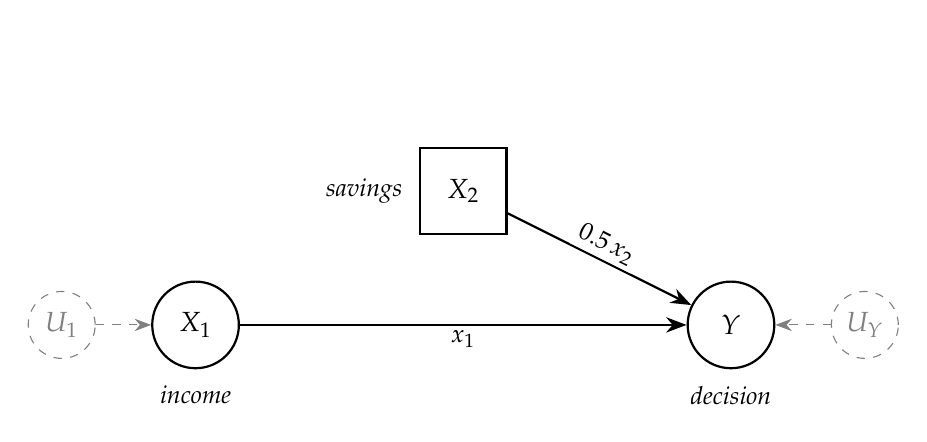
\begin{tikzpicture}[
    var/.style   = {circle, draw, thick, minimum size=11mm, inner sep=0pt},
    noise/.style = {circle, draw, dashed, gray, text=gray, minimum size=8.5mm, inner sep=0pt},
    intervened/.style = {rectangle, draw, thick, minimum size=11mm, inner sep=0pt},
    arr/.style   = {-{Stealth[length=2.6mm]}, thick},
    narr/.style  = {-{Stealth[length=2.1mm]}, dashed, gray},
    lab/.style   = {font=\small, fill=white, inner sep=1.5pt},
    word/.style  = {font=\small\itshape}
  ]
  \node[var]   (I)  at (0, 0)     {$X_1$};
  \node[intervened]   (S)  at (3.4, 1.7) {$X_2$};
  \node[var]   (Y)  at (6.8, 0)   {$Y$};
  \node[noise] (UI) at (-1.7, 0)  {$U_1$};
  \node[noise] (UY) at (8.5, 0)   {$U_Y$};
  \node[noise, draw=none] at (3.4, 3.35) {};   % invisible, where U_2 was

  \draw[arr] (S) -- node[lab, sloped, above] {$0.5\,x_2$} (Y);
  \draw[arr] (I) -- node[lab, below] {$x_1$} (Y);
  \draw[narr] (UI) -- (I);
  \draw[narr] (UY) -- (Y);

  \node[word, below=6.5mm] at (I) {income};
  \node[word, below=6.5mm] at (Y) {decision};
  \node[word, left=6.5mm]  at (S) {savings};
\end{tikzpicture}
\end{document}
